\documentclass{tufte-handout}
\usepackage{graphicx}
\usepackage{exercise}
\usepackage{enumerate}
\usepackage{amsmath,amssymb,amsthm}
\usepackage{enumitem}
%\usepackage{subcaption}
\usepackage{caption}
\usepackage{float}
\usepackage{hyperref}
\hypersetup{
    colorlinks = true,
    linkbordercolor = {white},
}
\usepackage{tikz}
\usepackage[numbered, framed]{matlab-prettifier}

% Silence warnings from tufte-handout bibliography handling
\usepackage{silence}
\WarningFilter{latex}{File `dummy.bib'}
\begin{filecontents*}{dummy.bib}
\end{filecontents*}
\WarningsOff[natbib]
\WarningsOff[bibentry]
\bibliographystyle{plainnat}

\newcommand{\bi}{\begin{itemize}}
\newcommand{\ei}{\end{itemize}}
\newcommand{\be}{\begin{enumerate}}
\newcommand{\ee}{\end{enumerate}}
\newcommand{\beq}{\begin{equation}}
\newcommand{\eeq}{\end{equation}}
\newcommand{\foo}[1]{%
\begin{tikzpicture}[#1]%
    \includegraphics[width=0.3cm]{figs/MatlabLogo.png}
\end{tikzpicture}%
}
\newcommand{\fuh}[1]{%
\begin{tikzpicture}[#1]%  x
    \includegraphics[width=0.3cm]{figs/MathematicaLogo.png}
\end{tikzpicture}%
}
\newcommand{\fie}[1]{%
\begin{tikzpicture}[#1]%
    \includegraphics[width=0.3cm]{figs/SolidworksLogo.png}
\end{tikzpicture}%
}
\let\ph\mlplaceholder % shorter macro
\lstMakeShortInline"

\lstset{
  style              = Matlab-editor,
  basicstyle         = \mlttfamily,
  escapechar         = ",
  mlshowsectionrules = true,
}


\title{Eigen Math \& Frequency Analysis for Audio}
\author{}
\date{\today}

\begin{document}

\maketitle

\vspace{0.1in}

% ----- Learning Goals -----
\section{Learning Goals}

\begin{description}[font=$\bullet$\scshape\bfseries]

\item[]Understand the difference between correlation and covariance matrix and how they are applied in different situations. 

\item[]Understand what singular vector decomposition yields and learn how to implement SVD in MATLAB.

\item[]Apply the knowledge from facial recognition and implement for voice classification via MATLAB.

\item[]Be able to conduct processing audio data in MATLAB.

\item[]Understand the complex math concept from external sources, such as academic paper.
\end{description}


% ----- Eigen-Math Review -----

\section{Eigen Analysis Revisited (3 hours)}

\subsection{What did we learn?}
During QEA I Module II, we learned how to recognize faces by conducting Principal Component Analysis, also known as Eigenfaces method. Basic idea for voice recognition works in similar fashion: a voice can be classified based on its variation from the entire mean of the voice data. Since \textbf{variance} can be also interpreted as the distance, or difference from the mean of the data, we can apply the same math from Module II for recognizing voices, such as Singular Vector Decomposition. Since it has been to long from middle of the first semester, we will review mathematical concept. 

\subsection{Principal Component Analysis - Correlation and Covariance}
Principal Component Analysis (PCA) uses an orthogonal transformation to convert a data set to a set of values of linearly uncorrelated variables called principal components.The number of distinct principal components is equal to the smaller of the number of original variables or the number of observations minus one (N-1). The transformation is defined that the first principal component has the largest possible variance, second principal component has the second largest possible variance and so on. Since the components are orthogonal to the preceding components, the resulting vectors are an uncorrelated orthogonal basis set. PCA is sensitive to the relative scaling of the original variables. Conducting PCA can be done by eigenvalue decomposition of a data covariance or correlation matrix or singular value decomposition of a data matrix, usually after mean centering (and normalizing) the data matrix for each elements. (\href{https://en.wikipedia.org/wiki/Principal_component_analysis}{Referenced})

A correlation matrix is a matrix showing correlation coefficients between sets of variables. Higher correlation coefficients mean two different data tips are more related to each other. Therefore, if a data matrix is defined as following:

\[
\textbf{Data} = 
\begin{bmatrix}
    x_{1} & y_{1}  \\
    x_{2} & y_{2}  \\
    \vdots & \vdots \\
    x_{n} & y_{n} 
\end{bmatrix}
\]
The correlation matrix is:
\[
\textbf{Correlation Matrix(A)}= 
\frac{1}{\sqrt{N}}
\begin{bmatrix}
    \frac{x_{1}-\mu_{x}}{\sigma_{x}}  & \frac{y_{1}-\mu_{y}}{\sigma_{y}} \\
    \frac{x_{2}-\mu_{x}}{\sigma_{x}} & \frac{y{2}-\mu_{y}}{\sigma_{y}} \\
    \frac{x_{3}-\mu_{x}}{\sigma_{x}} & \frac{y_{3}-\mu_{y}}{\sigma_{y}} \\
    \dots  & \dots
\end{bmatrix}
\]
\begin{marginfigure}
    \centering
    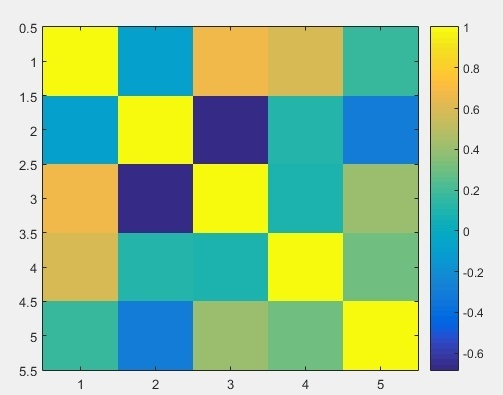
\includegraphics[width = 4cm, height = 4cm]{correlation.jpg}
    \label{fig:corr}
\caption{Example of Correlation Matrix Plot}
(\href{https://www.quora.com/Whats-the-best-way-to-visualize-correlations-between-six-value-vectors}{Referenced})


\end{marginfigure}

Where N is the number of rows in the matrix, $\mu_{x}, \mu_{y}$ are the mean of the data set, and $\sigma_{x}, \sigma_{y}$ are the standard deviation of the each column. 

A covariance matrix is a matrix built of covariance coefficients, which are the measures of how changes in one variable are associated with changes in a second variable. Essentially, covariance coefficient indicates the degree of linear association between two variables. Therefore, covariance matrix can be defined as

\[
\textbf{Covariance Matrix(B)}= 
\frac{1}{N-1}
\begin{bmatrix}
    (x_{1}-\mu_{1})(x_{1}-\mu{1})  & (y_{1}-\mu_{1})(y_{1}-\mu{1}) \\
    (x_{2}-\mu_{2})(x_{1}-\mu{1}) & (y_{2}-\mu_{2})(x_{2}-\mu{2}) \\
        \dots  & \dots \\
    (x_{n}-\mu_{n})(x_{1}-\mu{1}) & (y_{n}-\mu_{n})(y_{1}-\mu{2}) 

\end{bmatrix}
\]

\begin{marginfigure}
    \centering
    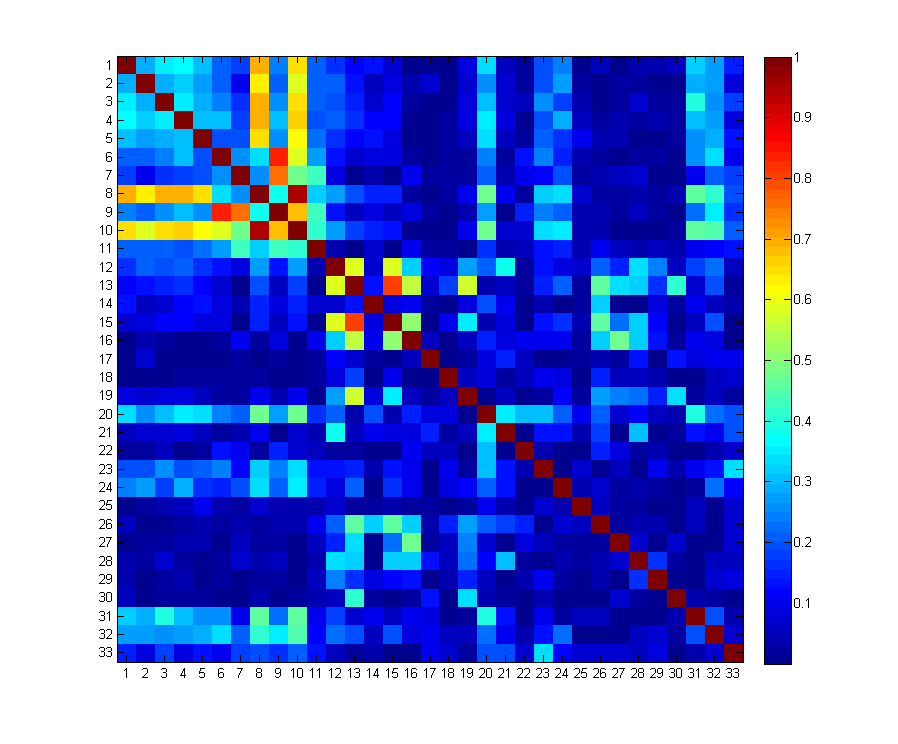
\includegraphics[width = 5cm, height = 4cm]{cov.png}
    \label{fig:cov}
\caption{Example of Covariance Matrix Plot}
(\href{https://www.mathworks.com/matlabcentral/answers/196574-factor-analysis-a-covariance-matrix-is-not-positive-definite}{Referenced})

\end{marginfigure}

Then, how should we choose what matrix to use for Principal Component Analysis? Covariance matrix is commonly used when variables are on the same scale. If the variables are on different scale, correlation matrix is used. For example, if the variables have different units of measure, such as pounds and inches. Since you cannot compare pounds and inches directly, you should use correlation matrix. If you want to conduct PCA on the temperature data for different cities, since the units of measure are the same (Either Fahrenheit or Celsius), covariance matrix should be used. In cases where scales are different, covariance matrix can also adjust the scales of the variables. For example, if you want to conduct PCA on population for different states, using covariance matrix would account for the size of each states.

\textit{Exercise 1}

Load sample data in MATLAB by typing \textit{load hospital}. Then, with \textit{[X = hospital.Weight, hospital.BloodPressure]}, plot the correlation and covariance matrix of the data and find how weight and blood pressure are related. Also, state how correlation and covariance matrix are different.

\begin{marginfigure}
    \centering
    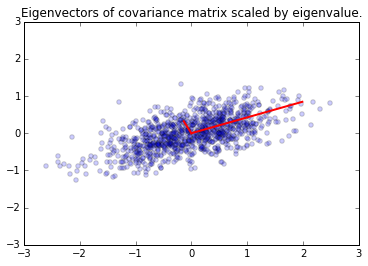
\includegraphics[width = 5cm, height = 4cm]{PCA.png}
    \label{fig:PCA}
\caption{Example of PCA}
(\href{https://people.duke.edu/~ccc14/sta-663/PCASolutions.html}{Referenced})

\end{marginfigure}

\subsection{Principal Component Analysis - Singular Value Decomposition}
Helpful Resource: 
\href{https://www.cs.cmu.edu/~venkatg/teaching/CStheory-infoage/book-chapter-4.pdf}{CMU CS Theory}

Singular Value decomposition is decomposition of a matrix M (m by n) whose entries come from the field K, which is either the field of real numbers or the field of complex numbers. The decomposition takes the form of ${\displaystyle \mathbf {M} =\mathbf {U} {\boldsymbol {\Sigma }}\mathbf {V} ^{*}}$, where $\mathbf{U}$ is m by m unitary matrix (if  K = ${\displaystyle \mathbb {R} } \mathbb {R}$ , unitary matrices are orthogonal matrices), $\boldsymbol{{\Sigma}}$ is a diagonal m by n matrix with non-negative real numbers on the diagonal, $\mathbf{V}$ is an n by n unitary matrix over K, and
$\mathbf{{V}^{*}}$ is the conjugate transpose of V.

The diagonal entries ${\sigma_{i}}$ of $\mathbf{\Sigma}$ are known as the singular values of M. A common convention is to list the singular values in descending order. In the other words, the first entry of the singular value (eigenvalue) represents how much of eigenvector corresponding to the eigenvalue is represented in the data. The second entry of the singular value represents the second most eminent direction how data is projected and so on. Therefore, by picking certain number of singular value, you can scale your data set and this process is called Principal Component Analysis. (\href{https://en.wikipedia.org/wiki/Singular-value_decomposition}{Referenced})



\textit{Exerise 2}

Load sample data in MATLAB by typing \textit{load hald}. Conduct SVD on one of four variables and plot the resultant data. These resources might be helpful: \href{https://www.mathworks.com/help/matlab/ref/svd.html}{SVD MATLAB documentation} and \href{http://www.matrixlab-examples.com/singular-value-decomposition.html}{SVD MATLAB tutorial}



% ----- Audio Preprocessing -----

\section{Frequency Analysis and Filtering (3 hours)}

\begin{marginfigure}
Insert margin figures here
\caption{caption here}
\end{marginfigure}

\subsection{Discrete Fourier Transform (DFT)}
*This section reviews and builds off section of the overnight from Module 2 Night 3.

Key ideas reviewed:
\begin{itemize}
	\item You can sample a continuous, real-world signal by sampling at discrete time steps using a simple matrix
	\item You can use these more simple, digital responses to analyze a signal
	\item You can convert a signal in the frequency domain back to the time domain
\end{itemize}

Recall that when a computer (or any digital device) samples an audio source, it samples it at a set frequency, or sampling rate. Basically a computer has a special type of clock in it that allows it to perform sampling operations only a certain number of times during a period of time. 

\begin{figure}
	\centering 
	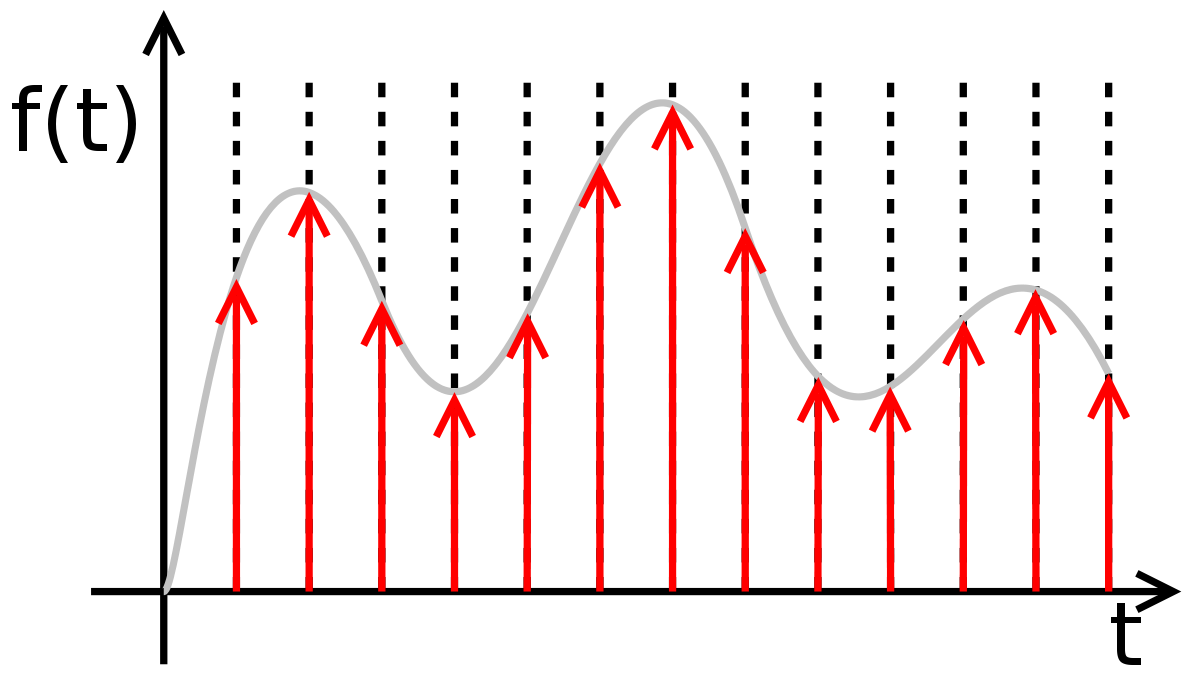
\includegraphics[width=0.7\textwidth]{discrete_time.png}
	\caption{\smaller{A continuous signal (in grey) being sampled at a specified sample rate (red arrows).}}
	\label{fig:discrete_time}
\end{figure}

As in figure \ref{fig:discrete_time}, a continuous sound signal can be broken up, or sampled, at different points. As you can imagine, if you don't sample at a high enough frequency, you will lose valuable information about your continuous signal. This is called aliasing. As you also might remember, as per the \textit{Nyquist Sampling Theorem}, you only have to sample at twice the frequency of the highest frequency present in your continuous signal to be able to fully reconstruct your continuous signal. 

Once you have turned a analog, continuous signal into a digital, discrete signal in the time domain, you can project it into the frequency domain which allows for rich analysis of the information within the signal. 

If you'd like to watch a quick (4 minutes) refresher video on the DFT, \href{https://www.youtube.com/watch?v=h6QJLx22zrE}{here} is a good video that explains how it works.

Recall that the Discrete Fourier Transform (DFT) works by taking a signal and sampling at a certain frequency $Fs$ and then correlating how much of each sinusoidal basis function is in each sample. 

Let's say our sampled signal looks like \ref{eq:sampled_audio} where $N$ is the time where the signal was sampled:
\begin{equation}\label{eq:sampled_audio}
    x=
\begin{bmatrix}
    x[1]       \\
    x[2]       \\
    \vdots \\
    x[N-1]
\end{bmatrix}
\end{equation}

Now we need to generate a matrix of the sinusoidal basis functions which are all just sinusoidal functions that are dependent on how many samples were taken and were they are in the sample range.
\begin{equation}\label{eq:basis_fns}
    W=\dfrac{1}{\sqrt{N}}
\begin{bmatrix}
    1 & 1 & 1 & \dots  & 1 \\
    1 & \exp(-\frac{2 \pi j}{N})2 & \exp(-\frac{2 \pi j}{N})3 & \dots  & \exp(-\frac{2 \pi j}{N})(N-1) \\
    1 & \exp(-\frac{3 \pi j}{N})2 & \exp(-\frac{2 \pi j}{N})3 & \dots  & \exp(-\frac{2 \pi j}{N}) (N-1) \\
    \vdots & \vdots & \vdots & \ddots & \vdots \\
    1 & \exp(-\frac{(N-1) \pi j}{N})2 & \exp(-\frac{(N-1) \pi j}{N})3 & \dots  & \exp(-\frac{(N-1) \pi j}{N}) (N-1)
\end{bmatrix}
\end{equation}
This vector can then be used to calculate the weights of $W$ on $x$ as
\begin{equation}
a = W x
\end{equation}
Once you get these weights, you can plot them and see the frequency response of the signal in the frequency domain. This is what the \textit{fft()} function does in Matlab.

To covert the signal back to time domain, you can use a similar matrix and the weights to get time function components. 
\begin{equation}\label{eq:basis_fns}
    W^{-1}=\dfrac{1}{\sqrt{N}}
\begin{bmatrix}
    1 & 1 & 1 & \dots  & 1 \\
    1 & \exp(\frac{2 \pi j}{N})2 & \exp(\frac{2 \pi j}{N})3 & \dots  & \exp(\frac{2 \pi j}{N})(N-1) \\
    1 & \exp(\frac{3 \pi j}{N})2 & \exp(\frac{2 \pi j}{N})3 & \dots  & \exp(\frac{2 \pi j}{N}) (N-1) \\
    \vdots & \vdots & \vdots & \ddots & \vdots \\
    1 & \exp(\frac{(N-1) \pi j}{N})2 & \exp(\frac{(N-1) \pi j}{N})3 & \dots  & \exp(\frac{(N-1) \pi j}{N}) (N-1)
\end{bmatrix}
\end{equation}

\subsection{Band Pass Filtering}

\subsection{Spectral Subtraction}


% ----- Spectral Subtraction -----

\section{Audio Preprocessing (2 hours)}

\begin{marginfigure}
Insert margin figures here
\caption{caption here}
\end{marginfigure}

%Length Matching

% Applying Filters

\subsection{Apply Eigen and Frequency analysis to audio}
% Finding Average Face

% Go further

\end{document}



